\documentclass[12pt,a4paper]{report}
\usepackage[utf8]{inputenc}
\usepackage[T1]{fontenc}
\usepackage[english]{babel}
\usepackage{geometry}
\usepackage{graphicx}
\usepackage{amsmath}
\usepackage{amssymb}
\usepackage{booktabs}
\usepackage{array}
\usepackage{multirow}
\usepackage{listings}
\usepackage{xcolor}
\usepackage{hyperref}
\usepackage{float}
\usepackage{caption}
\usepackage{subcaption}
\captionsetup{font=footnotesize} % 10pt for captions - required by regulations
\usepackage{tikz}
\usetikzlibrary{shapes.geometric, arrows, positioning}

% Line spacing - required by university regulations
\usepackage{setspace}
\onehalfspacing % 1.5 line spacing

\geometry{
    top=2.5cm,
    bottom=2.5cm,
    inner=3cm,
    outer=2cm,
    headheight=1.25cm,
    footskip=1.25cm,
    twoside % Enable mirror margins for double-sided printing
}

% Chapter/Section title formatting - required by university regulations
\usepackage{titlesec}

% Chapter titles (Level I) - 16pt, bold
\titleformat{\chapter}[display]
{\normalfont\bfseries\fontsize{16}{19}\selectfont}
{\chaptertitlename\ \thechapter}{20pt}{\bfseries\fontsize{16}{19}\selectfont}

% Section titles (Level II) - 14pt, bold
\titleformat{\section}
{\normalfont\bfseries\fontsize{14}{17}\selectfont}
{\thesection}{1em}{}

% Subsection titles (Level III) - 13pt, bold
\titleformat{\subsection}
{\normalfont\bfseries\fontsize{13}{16}\selectfont}
{\thesubsection}{1em}{}

% Page numbering - required by university regulations
\usepackage{fancyhdr}
\pagestyle{fancy}
\fancyhf{} % Clear all header/footer
\fancyfoot[LE,RO]{\fontsize{12}{14}\selectfont\thepage} % Left on even, right on odd
\renewcommand{\headrulewidth}{0pt} % No header line
\renewcommand{\footrulewidth}{0pt} % No footer line

% Paragraph formatting - recommended by university regulations
\setlength{\parindent}{0.5cm}
\setlength{\parskip}{0pt}

% Code listing style
\lstset{
    basicstyle=\ttfamily\small,
    breaklines=true,
    frame=single,
    numbers=left,
    numberstyle=\tiny,
    keywordstyle=\color{blue},
    commentstyle=\color{green!60!black},
    stringstyle=\color{red},
    showstringspaces=false
}

\title{
    \textbf{Implementation of Convolutional Neural Network on FPGA for MNIST Digit Recognition}\\[1cm]
    \large Engineering Thesis
}
\author{}
\date{}

\begin{document}

\maketitle

\tableofcontents
\newpage

%==============================================================================
% ABSTRACT
%==============================================================================
\begin{abstract}
In the early days of artificial intelligence, neural networks were primarily trained on CPUs, which lacked the necessary power for deep architectures. The 2012 debut of AlexNet marked a turning point by leveraging the massive parallelism of GPUs to significantly accelerate matrix operations. However, the high energy demands of GPUs have driven a shift toward more efficient hardware, such as FPGAs and ASICs, to optimize inference for embedded systems.

This thesis presents a complete end-to-end implementation of a LeNet-5 for MNIST handwritten digit classification on a Basys3 FPGA board featuring the Xilinx Artix-7 XC7A35T chip. The project encompasses three main components: (1) training a LeNet-5 CNN model using PyTorch with post-training static quantization to 8-bit integers, (2) implementing the inference engine in Verilog RTL as a 44-state finite state machine with specialized BRAM latency handling, and (3) comprehensive verification through Python simulation and hardware testing via UART communication.

Key features include a complete quantization pipeline that preserves accuracy while enabling efficient fixed-point arithmetic, a modular RTL architecture using hybrid memory (distributed RAM for activation buffers, Block RAM for weight storage), and a robust UART protocol for weight loading and real-time inference. The implementation demonstrates the viability of deploying neural networks on resource-constrained FPGAs for embedded applications.

The system achieves 97.6\% classification accuracy after quantization while maintaining bit-exact correspondence between Python simulation and FPGA hardware inference.

\textbf{Keywords:} FPGA, CNN, MNIST, Quantization, Verilog
\end{abstract}

\newpage

%==============================================================================
% CHAPTER 1: INTRODUCTION
%==============================================================================
\chapter{Introduction}

\section{Background and Motivation}

Deep neural networks demand extraordinary computational resources, performing billions of multiply-accumulate operations for a single inference. Traditional CPU architectures proved inadequate for such workloads, prompting the exploration of specialized accelerators. The watershed moment arrived in 2012 when AlexNet demonstrated that Graphics Processing Units could dramatically accelerate deep learning training through massively parallel processing, achieving breakthrough performance on the ImageNet classification challenge \cite{alexnet}. This discovery catalyzed widespread adoption of GPUs for neural network development, fundamentally reshaping the AI research landscape and enabling the deep learning revolution.

Despite their training dominance, GPUs face significant challenges in deployment scenarios. Power consumption exceeding 200 watts, substantial physical size, and high cost make GPUs impractical for embedded and edge applications. Field-Programmable Gate Arrays have emerged as compelling alternatives for neural network inference, offering reconfigurable hardware that bridges the gap between software flexibility and hardware efficiency \cite{fpga_cnn_survey}. FPGAs provide distinct advantages: energy consumption in single-digit watts, deterministic latency for real-time systems, support for custom bit-width arithmetic enabling aggressive quantization, and the ability to implement application-specific datapaths. These characteristics make FPGAs particularly suitable for resource-constrained deployments in autonomous systems, industrial automation, telecommunications infrastructure, and aerospace applications where power efficiency and reliability are paramount.

\section{Scope of the Thesis}

This work demonstrates a complete implementation of the classic LeNet-5 convolutional neural network for MNIST digit classification on the Xilinx Artix-7 XC7A35T FPGA (Digilent Basys3 board). The system integrates three components: PyTorch-based training with post-training quantization to 8-bit integers, Verilog RTL inference engine implemented as a 44-state finite state machine with dedicated BRAM latency handling, and comprehensive verification ensuring bit-exact correspondence between software simulation and hardware execution. The LeNet-5 architecture processes 28$\times$28 grayscale images through two convolutional layers (with 5$\times$5 kernels), average pooling, and three fully-connected classification layers, with all weights and activations quantized to enable efficient fixed-point arithmetic on FPGA fabric. \cite{lecun1998}
Implementation highlights include a complete quantization workflow that accounts for scale propagation through average pooling layers while preserving classification accuracy, a modular RTL design utilizing distributed RAM for convolutional layers and Block RAM for fully-connected weights, a 256-entry tanh lookup table for activation functions, and a robust UART-based protocol for weight loading and real-time inference control. The implementation achieves 97.6\% accuracy on MNIST classification (bit-exact match with quantized Python model) and matches floating-point PyTorch accuracy with zero degradation. These results validate FPGA-based neural network deployment as viable for embedded applications where power efficiency and deterministic latency are critical requirements.

\section{Historical Context}

LeNet-5 is a pioneering convolutional neural network architecture developed by Yann LeCun and colleagues in the 1990s for handwritten digit recognition. This architecture established several fundamental principles that remain relevant in modern deep learning:

\begin{itemize}
    \item \textbf{Local Receptive Fields:} Small convolutional kernels that detect local features
    \item \textbf{Weight Sharing:} The same kernel applied across the entire input, reducing parameters
    \item \textbf{Subsampling (Pooling):} Spatial dimension reduction for translation invariance
    \item \textbf{Hierarchical Feature Extraction:} Progressive abstraction from edges to digits
\end{itemize}

What distinguishes LeNet-5 from classical machine learning models such as decision trees, random forests, and support vector machines is its ability to automatically learn hierarchical feature representations directly from raw pixel data. Traditional machine learning approaches require manual feature engineering—extracting handcrafted features like edge histograms, Histogram of Oriented Gradients (HOG), or Scale-Invariant Feature Transform (SIFT) descriptors—before classification can occur. LeNet-5 eliminates this bottleneck through end-to-end learning, where convolutional layers progressively discover optimal features during training, from low-level edges to high-level digit shapes. This architectural advantage, combined with inherent translation invariance through pooling, enables LeNet-5 to achieve superior accuracy on image classification tasks while requiring minimal domain expertise in feature design.

LeNet-5 originally employed average pooling and tanh activations, design choices that proved highly effective for the MNIST digit classification task. 

%==============================================================================
% CHAPTER 2: THEORETICAL FOUNDATIONS
%==============================================================================
\chapter{Theoretical Foundations}

This chapter provides essential background on the key technologies relevant to neural network deployment on reconfigurable hardware: Field-Programmable Gate Arrays, Convolutional Neural Networks, serial communication protocols, and quantization techniques.

\section{Field-Programmable Gate Arrays}

A Field-Programmable Gate Array (FPGA) is a semiconductor device containing configurable logic blocks that can be programmed after manufacturing to implement custom digital circuits. Unlike Application-Specific Integrated Circuits (ASICs) with fixed functionality or general-purpose processors (CPUs, GPUs) that execute software instructions, FPGAs offer a middle ground: hardware-level performance with post-fabrication reconfigurability.

FPGAs implement computation through \textbf{spatial parallelism}—operations execute simultaneously across physically distributed logic rather than sequentially through shared arithmetic units. This architectural difference provides several advantages: deterministic latency without caches or branch prediction, custom bit-width arithmetic (e.g., 8-bit integers instead of 32-bit floats), and power efficiency typically in single-digit watts compared to 200+ watts for high-performance GPUs. These characteristics make FPGAs particularly suitable for embedded neural network inference where power constraints and real-time guarantees are critical.

Modern FPGAs contain three primary resource types: \textbf{Look-Up Tables (LUTs)} implement combinational logic by storing truth tables in SRAM; \textbf{Flip-Flops} provide clocked storage for sequential circuits; and \textbf{Block RAM} offers dedicated memory blocks for data storage. Memory architecture significantly impacts performance—Block RAM provides high capacity but introduces multi-cycle read latency, while distributed RAM (LUT-based) enables single-cycle access at the cost of consuming logic resources. The choice between memory types affects state machine design and overall throughput (as demonstrated in this work's LeNet-5 implementation on Artix-7).

\section{Convolutional Neural Networks}

Convolutional Neural Networks are deep learning architectures designed for processing grid-structured data, particularly images. The fundamental innovation is \textbf{weight sharing}: instead of connecting every input pixel to every output neuron (as in fully-connected networks), CNNs apply small learnable filters repeatedly across the input, dramatically reducing parameter counts while preserving spatial relationships.

Three core operations define CNNs, illustrated using LeNet-5 as an example (see Figure~\ref{fig:lenet5_architecture} in Section~3.1):

\textbf{Convolution} slides filters (typically 3$\times$3 or 5$\times$5 kernels) across the input, computing dot products at each position to detect local patterns like edges or textures. As an example, the LeNet-5 architecture (detailed in Figure~\ref{fig:lenet5_architecture}, Section~3.1) processes 32$\times$32 input images, but this implementation adapts it for native 28$\times$28 MNIST images. To preserve spatial dimensions when applying 5$\times$5 kernels, \textbf{padding} is employed—adding 2 pixels of zeros on each border effectively expands 28$\times$28 to 32$\times$32 before convolution. This allows the kernel to operate on edge pixels: when centered at the top-left corner (0,0) of the original image, the 5$\times$5 kernel extends into the padded border, ensuring all original pixels receive equal receptive field coverage. Without padding, a 5$\times$5 kernel on 28$\times$28 input would produce only 24$\times$24 output, losing spatial information at boundaries.

\textbf{Pooling} (labeled as S2 and S4 in the LeNet-5 example, Figure~\ref{fig:lenet5_architecture}) downsamples feature maps by applying reduction functions (max or average) over windows, providing limited translation invariance and reducing spatial dimensions. After the first convolutional layer produces 28$\times$28 feature maps, 2$\times$2 average pooling with stride 2 reduces them to 14$\times$14, halving both dimensions.

\textbf{Activation functions} introduce nonlinearity—historically tanh or sigmoid, now predominantly ReLU ($\max(0, x)$) \cite{relu}—enabling networks to learn complex, non-linear decision boundaries. This implementation uses tanh activation after each convolutional and fully-connected layer, matching the original LeNet-5 design.

LeNet-5, developed by Yann LeCun in 1998 for handwritten digit recognition, established the canonical CNN architecture pattern (see detailed architecture diagram in Figure~\ref{fig:lenet5_architecture}, Section~3.1): alternating convolutional/pooling layers (C1-S2-C3-S4) for hierarchical feature extraction, followed by fully-connected layers (C5-F6-OUTPUT) for classification. Despite its age, LeNet-5 remains pedagogically valuable due to its simplicity (61,706 parameters, 416,520 multiply-accumulate operations per inference) while demonstrating core principles applicable to modern architectures like ResNet and EfficientNet.

\section{Serial Communication Protocols}

Serial communication transmits data sequentially over a single wire or differential pair, trading throughput for reduced pin count and board complexity compared to parallel buses. UART (Universal Asynchronous Receiver-Transmitter) is the most common asynchronous serial protocol, requiring no shared clock between transmitter and receiver. Instead, both sides agree on a baud rate (bits per second) in advance, and the receiver synchronizes on start bits marking each byte transmission.

For applications transmitting structured data (e.g., neural network weights), higher-level protocols use marker sequences to delimit packets. A key challenge is \textbf{binary-safe detection}: marker bytes may appear in arbitrary data payloads, requiring payload-length-aware parsing to prevent false packet termination.

\begin{figure}[H]
\centering
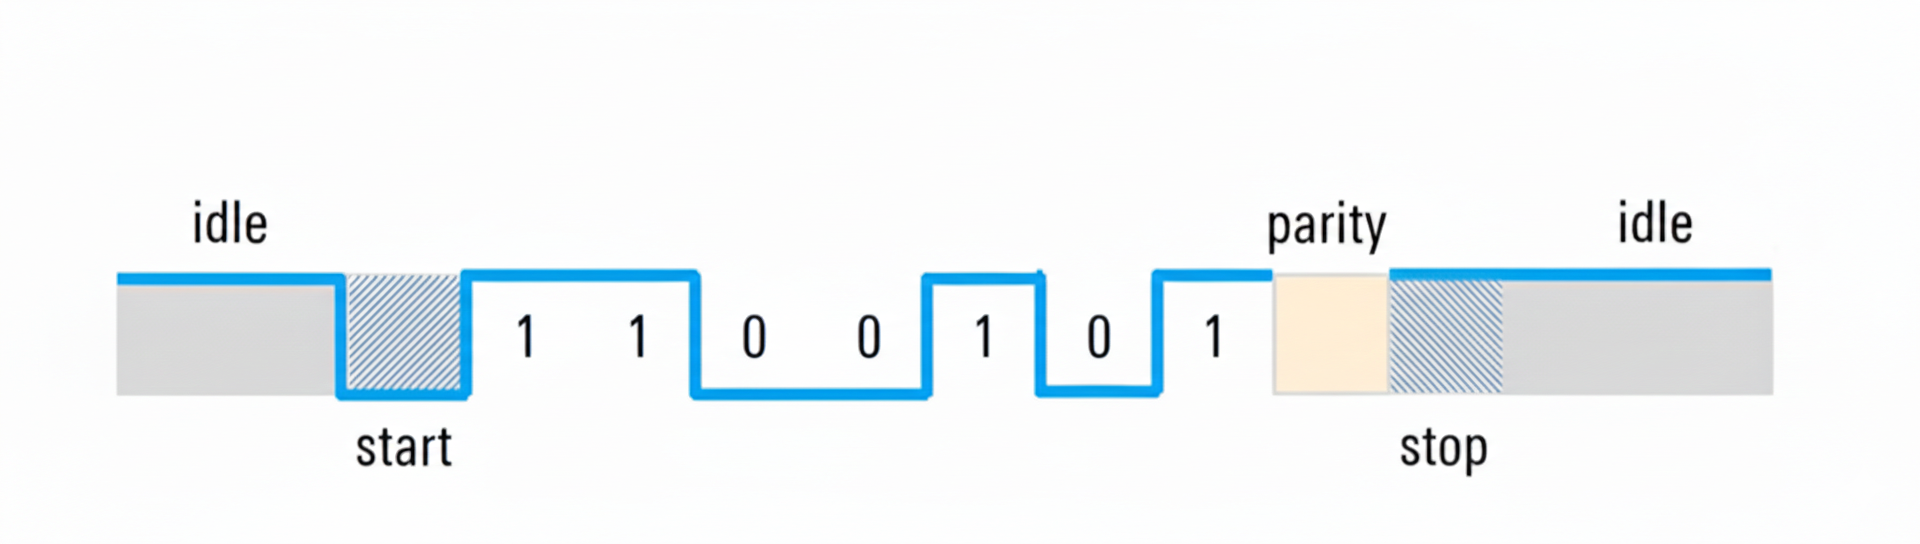
\includegraphics[width=0.9\textwidth]{UART.png}
\caption{UART 8N1 Frame Format}
\label{fig:uart_waveform}
\end{figure}

The standard UART frame format (8N1) consists of: 1 start bit (falling edge), 8 data bits transmitted LSB-first, no parity, and 1 stop bit (return to idle high). The first falling edge from idle high to low marks the \textbf{start bit}, which triggers the receiver to synchronize and begin sampling data bits at the agreed baud rate. Following the start bit, 8 data bits are transmitted sequentially, least significant bit (LSB) first. The \textbf{parity bit} is an optional error-checking mechanism (P = even/odd parity, N = no parity); in 8N1 format, no parity bit is included. After the data bits, the \textbf{stop bit} returns the line to the idle high state, signaling the end of the frame.

Figure~\ref{fig:uart_waveform} illustrates the transmission of ASCII character 'S' (0x53 = 01010011 in binary). Due to LSB-first transmission, the bit sequence on the wire is reversed: 1-1-0-0-1-0-1-0. At 115,200 baud—a common rate for microcontroller/FPGA communication—each bit period is 8.68 microseconds, resulting in a complete 10-bit frame time of approximately 87 microseconds and maximum throughput of 11.5 KB/second.

\section{Neural Network Quantization}

Quantization reduces neural network computational, time needed for arithmetic operations and memory requirements by converting floating-point parameters to lower-precision fixed-point representations \cite{ptq_fpga}. \textbf{Post-training quantization} applies after training completes, mapping FP32 weights to INT8 via scale factors $W_{\text{scale}} = 127 / \max(|W|)$. Biases typically require higher precision (INT32) to prevent overflow during accumulation. The quantization introduces rounding error but often preserves accuracy—for MNIST classification, a drop can be minimized to less than 1\% compared to the FP32 baseline.

Hardware implementations benefit substantially from quantization: INT8 multipliers consume far less area and power than FP32 units, and reduced memory footprint enables deployment on resource-constrained devices. The inference pipeline typically accumulates multiply-accumulate products in higher precision (INT32), then applies scaling (arithmetic right shift), activation, and saturation back to INT8. Verification requires bit-exact simulation to ensure hardware arithmetic matches the quantized software model across all test cases.

%==============================================================================
% CHAPTER 3: TRAINING
%==============================================================================
\chapter{Training}

This chapter describes the training pipeline for the LeNet-5 model, including the neural network architecture, dataset preparation, training process, and the critical quantization strategy that enables efficient FPGA implementation.

\section{LeNet-5 Architecture}

\begin{figure}[H]
\centering
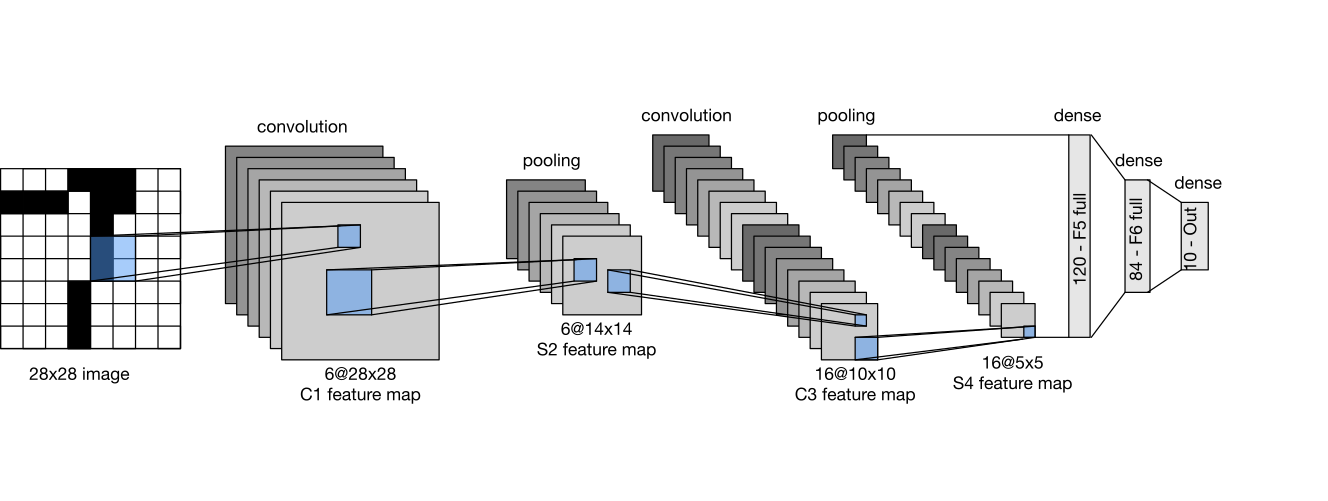
\includegraphics[width=0.9\textwidth]{../presentation/LeNet-5_architecture.png}
\caption{LeNet-5 Architecture \cite{lenet_image}}
\label{fig:lenet5_architecture}
\end{figure}

The implemented model is the classic LeNet-5 architecture (see Figure~\ref{fig:lenet5_architecture}) optimized for FPGA deployment. The network consists of two convolutional layers with average pooling, followed by three fully-connected layers for classification (detailed specifications are provided in Section~\ref{sec:lenet_mac_ops}).

\textbf{Convolutional Layer 1:}
\begin{itemize}
    \item 6 filters with $5 \times 5$ kernels
    \item Padding 2, stride 1
    \item Tanh activation
    \item Output: $6 \times 28 \times 28$
    \item Captures low-level features: edges, corners, curves
\end{itemize}

\textbf{Average Pooling Layer 1:}
\begin{itemize}
    \item $2 \times 2$ kernel, stride 2
    \item Output: $6 \times 14 \times 14$
    \item Subsampling for translation invariance
\end{itemize}

\textbf{Convolutional Layer 2:}
\begin{itemize}
    \item 16 filters with $5 \times 5$ kernels across 6 input channels
    \item No padding, stride 1
    \item Tanh activation
    \item Output: $16 \times 10 \times 10$
    \item Combines features into higher-level patterns
\end{itemize}

\textbf{Average Pooling Layer 2:}
\begin{itemize}
    \item $2 \times 2$ kernel, stride 2
    \item Output: $16 \times 5 \times 5$ = 400 features
    \item Further spatial reduction
\end{itemize}

\textbf{Fully Connected Layer 1:}
\begin{itemize}
    \item 400 input features from flattened pool output
    \item 120 output neurons
    \item Tanh activation
\end{itemize}

\textbf{Fully Connected Layer 2:}
\begin{itemize}
    \item 120 input features
    \item 84 output neurons
    \item Tanh activation
\end{itemize}

\textbf{Fully Connected Layer 3:}
\begin{itemize}
    \item 84 input features
    \item 10 output neurons (one per digit class)
    \item No activation (raw logits for classification)
\end{itemize}

\section{Dataset and Preprocessing}

\subsection{MNIST Dataset}

The MNIST database of handwritten digits \cite{mnist_dataset} contains:
\begin{itemize}
    \item 60,000 training images
    \item 10,000 test images
    \item Each image: $28 \times 28$ pixels, grayscale (0-255)
    \item 10 classes (digits 0-9)
\end{itemize}

\begin{figure}[H]
\centering

\includegraphics[width=0.3\textwidth]{mnist_sample.png}
\caption{Example MNIST handwritten digit \cite{mnist_dataset}}
\end{figure}

\subsection{Preprocessing Pipeline}

The preprocessing transforms raw pixel values for neural network input:

\begin{equation}
x_{normalized} = \frac{x_{raw}/255 - \mu}{\sigma}
\end{equation}

where $\mu = 0.1307$ and $\sigma = 0.3081$ are the MNIST dataset statistics.

For FPGA deployment, the normalized values are quantized to 8-bit signed integers:

\begin{equation}
x_{int8} = \text{clip}\left(\text{round}(x_{normalized} \times 127), -128, 127\right)
\end{equation}

\section{Training Configuration}

The model is trained using PyTorch \cite{pytorch} with the following hyperparameters:

\begin{table}[H]
\centering
\caption{Training Hyperparameters}
\begin{tabular}{ll}
\toprule
\textbf{Parameter} & \textbf{Value} \\
\midrule
Batch Size & 64 \\
Epochs & 10 \\
Learning Rate & 0.001 \\
Optimizer & Adam \\
Loss Function & Cross-Entropy \\
\bottomrule
\end{tabular}
\end{table}

\textbf{Batch Size} determines how many training samples are processed together before updating network weights—larger batches provide more stable gradient estimates but require more memory, while very small batches (e.g., 1) cause noisy updates that may prevent convergence, making the choice of 64 a practical balance between stability and computational efficiency. \textbf{Epochs} specify how many complete passes through the entire training dataset are performed—10 epochs means the network sees all 60,000 MNIST images 10 times. \textbf{Learning Rate} controls the step size during weight updates—smaller values (0.001) ensure stable convergence but slower training. \textbf{Optimizer} defines the weight update algorithm—Adam (Adaptive Moment Estimation) adapts learning rates per parameter and combines momentum for faster convergence. \textbf{Loss Function} measures prediction error—Cross-Entropy compares predicted class probabilities against true labels, penalizing confident incorrect predictions more heavily.

\section{Quantization Strategy}

The project employs \textbf{post-training static quantization} to convert floating-point weights to integers while preserving accuracy. Post-training quantization (PTQ) was chosen over quantization-aware training (QAT) due to its simplicity in implementation, requiring no retraining or modification to the training pipeline. For this MNIST application, PTQ achieved approximately 1.3\% accuracy drop.

\subsection{Weight Quantization}

Weights are quantized to 8-bit signed integers:

\begin{equation}
W_{scale} = \frac{127.0}{\max(|W_{float}|)}
\end{equation}

\begin{equation}
W_{int8} = \text{clip}\left(\text{round}(W_{float} \times W_{scale}), -128, 127\right)
\end{equation}

\subsection{Bias Quantization}

Biases are quantized to 32-bit signed integers with scale propagation through layers:

\textbf{Layer 1:}
\begin{align}
\text{InputScale} &= 127.0 \\
\text{BiasScale}_{L1} &= \text{InputScale} \times W_{scale,L1} \\
\text{Bias}_{L1,int32} &= \text{round}(\text{Bias}_{L1,float} \times \text{BiasScale}_{L1})
\end{align}

\textbf{Layer 2 and Dense:}
\begin{align}
\text{OutputScale}_{L1} &= \frac{\text{InputScale} \times W_{scale,L1}}{2^{SHIFT}} \\
\text{BiasScale}_{L2} &= \text{OutputScale}_{L1} \times W_{scale,L2}
\end{align}

where $SHIFT$ varies per layer (Conv1=10, Conv2=8, FC1=9, FC2=10) to accommodate different input scales after average pooling and tanh activation.

\subsection{Arithmetic Pipeline}

The FPGA computes each convolution output as:

\begin{equation}
acc = bias + \sum_{i} (pixel_i \times weight_i)
\end{equation}

Followed by the scaling and activation pipeline:

\begin{enumerate}
    \item \textbf{Arithmetic Right Shift:} $temp = acc \gg SHIFT$ (per-layer shift value)
    \item \textbf{Clip to LUT range:} $temp = \text{clip}(temp, -128, 127)$
    \item \textbf{Tanh LUT index:} $idx = temp + 128$ (offset to unsigned 0-255)
    \item \textbf{Tanh activation:} $output = \text{tanh\_lut}[idx]$
\end{enumerate}

The per-layer SHIFT values account for different input scales throughout the network:

\begin{table}[H]
\centering
\begin{tabular}{lll}
\toprule
\textbf{Layer} & \textbf{SHIFT} & \textbf{Input Scale} \\
\midrule
Conv1 & 10 & 127.0 (normalized input) \\
Conv2 & 8 & 31.75 (post-pool, 127/4) \\
FC1 & 9 & 31.75 (post-pool) \\
FC2 & 10 & 127.0 (post-tanh) \\
\bottomrule
\end{tabular}
\end{table}

%==============================================================================
% CHAPTER 4: INFERENCE IMPLEMENTATION
%==============================================================================
\chapter{Inference Implementation}

This chapter describes the FPGA implementation of the CNN inference engine, including the hardware architecture, finite state machine design, memory organization, and communication protocols.

\section{Target Hardware}

The implementation targets the Digilent Basys3 development board \cite{basys3_manual}, featuring:

\begin{table}[H]
\centering
\caption{Target Hardware Specifications}
\begin{tabular}{ll}
\toprule
\textbf{Component} & \textbf{Specification} \\
\midrule
FPGA Chip & Xilinx Artix-7 XC7A35T-1CPG236C \\
Logic Cells & 33,280 \\
Block RAM & 1,800 Kbit (225 KB) \\
DSP Slices & 90 \\
System Clock & 100 MHz \\
UART Baud Rate & 115,200 bps \\
\bottomrule
\end{tabular}
\end{table}

The Artix-7 family represents a cost-effective, low-power FPGA option suitable for educational and embedded applications, making it an appropriate platform for demonstrating neural network inference in resource-constrained environments.

\section{System Architecture}

The top-level design follows a modular architecture:

\begin{figure}[H]
\centering
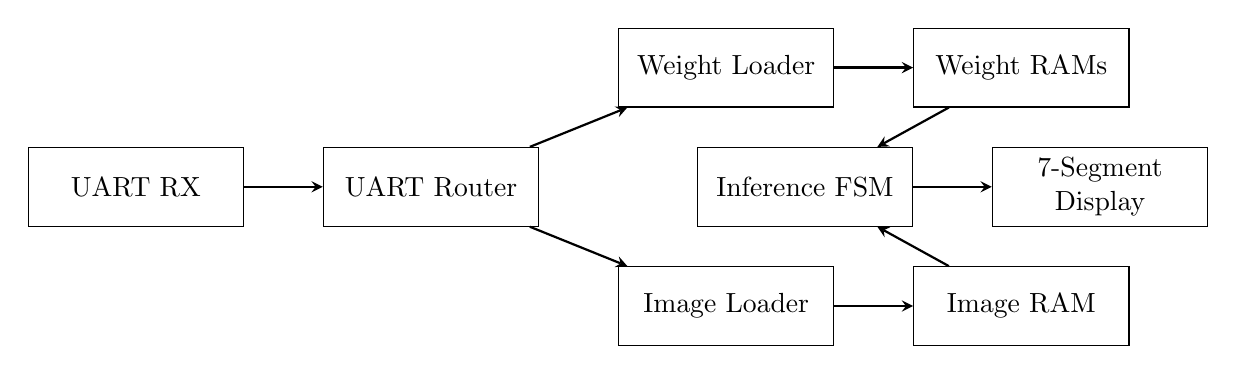
\begin{tikzpicture}[
    block/.style={rectangle, draw, text width=2.5cm, text centered, minimum height=1cm},
    arrow/.style={->, >=stealth, thick}
]
    % UART section
    \node[block] (uart_rx) {UART RX};
    \node[block, right=1cm of uart_rx] (uart_router) {UART Router};
    
    % Loaders
    \node[block, above right=0.5cm and 1cm of uart_router] (weight_loader) {Weight Loader};
    \node[block, below right=0.5cm and 1cm of uart_router] (image_loader) {Image Loader};
    
    % RAMs
    \node[block, right=1cm of weight_loader] (weight_rams) {Weight RAMs};
    \node[block, right=1cm of image_loader] (image_ram) {Image RAM};
    
    % Inference
    \node[block, right=2cm of uart_router] (inference) {Inference FSM};
    
    % Output
    \node[block, right=1cm of inference] (output) {7-Segment Display};
    
    % Arrows
    \draw[arrow] (uart_rx) -- (uart_router);
    \draw[arrow] (uart_router) -- (weight_loader);
    \draw[arrow] (uart_router) -- (image_loader);
    \draw[arrow] (weight_loader) -- (weight_rams);
    \draw[arrow] (image_loader) -- (image_ram);
    \draw[arrow] (weight_rams) -- (inference);
    \draw[arrow] (image_ram) -- (inference);
    \draw[arrow] (inference) -- (output);
\end{tikzpicture}
\caption{High-Level System Block Diagram}
\label{fig:system_architecture}
\end{figure}

Figure~\ref{fig:system_architecture} illustrates the complete FPGA inference pipeline, organized into three functional subsystems: the communication layer (UART RX, UART Router), the memory subsystem (Weight RAMs, Image RAM, working buffers), and the computation engine (Inference FSM). The modular architecture achieves clear separation of concerns, with each component fulfilling a specific role in the digit classification workflow. Data flows from the host PC through the UART interface, into dedicated memory structures, through the inference computation, and finally to the 7-segment display and optional result readback via UART TX.

The \textbf{communication layer} handles all data transfer between the host PC and FPGA. The UART RX module receives serial data at 115,200 baud using 8N1 format (8 data bits, no parity, 1 stop bit), which the UART Router then parses according to a binary-safe protocol using start/end marker sequences (0xAA 0x55 for weight packets, 0xBB 0x66 for image packets). The router implements payload-aware marker detection to prevent false end-marker detection within binary weight data, only validating end markers after receiving the complete expected payload (62,670 bytes for weights, 784 bytes for images). Based on the detected packet type, the router gates data to either the Weight Loader or Image Loader module, which then populate their respective memory structures.

The \textbf{memory hierarchy} stores all neural network parameters and working data required for inference. Weight RAMs store the complete set of 61,706 network parameters, including convolutional layer weights and biases (using distributed RAM for 0-cycle read latency), fully connected layer weights and biases (using Block RAM for higher density), and a 256-entry tanh lookup table for activation functions. Image RAM holds the 28$\times$28 preprocessed input pixels (784 bytes total). The system also employs three working buffers (Buffer A, B, and C) implemented in distributed RAM to store intermediate activations between layers, enabling the FSM to access data with single-cycle latency during computation. Each buffer is strategically reused across multiple layers: Buffer A stores Conv1 output (6$\times$28$\times$28) then Conv2 output (16$\times$10$\times$10), Buffer B stores Pool1 output (6$\times$14$\times$14) then FC1 output (120 neurons), and Buffer C stores Pool2 output (16$\times$5$\times$5) then FC2 output (84 neurons). This reuse is possible because the FSM processes layers sequentially—once a subsequent layer consumes data from a buffer, that data is no longer needed and the buffer can be overwritten. Multiple buffers are necessary because layers must simultaneously read input data while writing output results, preventing in-place updates to a single buffer.

The \textbf{Inference FSM} serves as the computational core, implementing a 44-state finite state machine that executes the complete LeNet-5 pipeline sequentially. The processing flow is: Conv1$\rightarrow$Pool1$\rightarrow$Conv2$\rightarrow$Pool2$\rightarrow$FC1$\rightarrow$FC2$\rightarrow$FC3. For each layer, the FSM orchestrates data fetching from appropriate memories, performs multiply-accumulate (MAC) operations using pure fixed-point integer arithmetic, applies tanh activation via lookup table where required, and stores results in working buffers. The complete inference executes 416,520 MAC operations per image, with the FSM managing different memory latencies (distributed RAM with 0-cycle latency versus Block RAM with 1-2 cycle latency) through carefully designed wait states. The final layer computes class scores for digits 0-9, with the FSM tracking the argmax to determine the predicted digit.

System operation follows a \textbf{two-phase protocol}. In Phase 1 (weight loading), the UART Router gates the Weight Loader to receive all 62,670 bytes of network parameters, then sets a \texttt{weights\_loaded} flag to indicate readiness. In Phase 2 (inference), the system accepts image packets (784 bytes each), triggering the Inference FSM to execute the complete forward pass. Results are stored in dedicated output memories: Scores RAM (40 bytes for ten 32-bit class scores) and Predicted Digit RAM (1 byte). The predicted digit is immediately displayed on the 7-segment display, while the host PC can optionally request results via UART commands (0xCC for predicted digit, 0xCD for all class scores). This gating mechanism prevents out-of-sequence operations and ensures the inference engine has valid weights before attempting classification.

The modular design enables independent development and testing of each component. Detailed specifications for subsystems are provided in subsequent sections: Section~\ref{sec:lenet_mac_ops} presents layer-by-layer computational requirements, Section~4.3 describes the Inference FSM state machine implementation, Section~4.4 explains the hybrid memory architecture and allocation strategy, and Section~4.5 specifies the complete UART communication protocol including binary packet formats.

\section{MAC Operations}
\label{sec:lenet_mac_ops}

This section provides detailed computational requirements for each layer of the LeNet-5 architecture, including parameter counts and multiply-accumulate (MAC) operations per inference.

\begin{table}[H]
\centering
\caption{LeNet-5 Layer Specifications}
\begin{tabular}{lllll}
\toprule
\textbf{Layer} & \textbf{Input Shape} & \textbf{Output Shape} & \textbf{Parameters} & \textbf{Operations} \\
\midrule
Input & -- & $1 \times 28 \times 28$ & 0 & -- \\
Conv1 & $1 \times 28 \times 28$ & $6 \times 28 \times 28$ & 156 & 117,600 MACs \\
AvgPool1 & $6 \times 28 \times 28$ & $6 \times 14 \times 14$ & 0 & -- \\
Conv2 & $6 \times 14 \times 14$ & $16 \times 10 \times 10$ & 2,416 & 240,000 MACs \\
AvgPool2 & $16 \times 10 \times 10$ & $16 \times 5 \times 5$ & 0 & -- \\
Flatten & $16 \times 5 \times 5$ & 400 & 0 & -- \\
FC1 & 400 & 120 & 48,120 & 48,000 MACs \\
FC2 & 120 & 84 & 10,164 & 10,080 MACs \\
FC3 & 84 & 10 & 850 & 840 MACs \\
\midrule
\textbf{Total} & & & \textbf{61,706} & \textbf{416,520 MACs} \\
\bottomrule
\end{tabular}
\end{table}

\textbf{Convolutional Layer 1:}
\begin{itemize}
    \item \textit{Parameters:} 6 output channels $\times$ (5$\times$5 kernel $\times$ 1 input channel + 1 bias) = 6 $\times$ (25 + 1) = 156
    \item \textit{MAC Operations:} 6 output channels $\times$ 28$\times$28 output positions $\times$ 5$\times$5 kernel operations
    \begin{equation}
    \text{MACs}_{Conv1} = 6 \times 784 \times 25 = 117,600
    \end{equation}
    Each output pixel requires 25 multiplications (5$\times$5 kernel) and 25 accumulations.
\end{itemize}

\textbf{Convolutional Layer 2:}
\begin{itemize}
    \item \textit{Parameters:} 16 output channels $\times$ (5$\times$5 kernel $\times$ 6 input channels + 1 bias) = 16 $\times$ (150 + 1) = 2,416
    \item \textit{MAC Operations:} 16 output channels $\times$ 10$\times$10 output positions $\times$ (5$\times$5 kernel $\times$ 6 input channels)
    \begin{equation}
    \text{MACs}_{Conv2} = 16 \times 100 \times 150 = 240,000
    \end{equation}
    Each output pixel requires 150 multiplications (5$\times$5$\times$6 kernel volume) across all input channels.
\end{itemize}

\textbf{Fully Connected Layer 1:}
\begin{itemize}
    \item \textit{Parameters:} 400 inputs $\times$ 120 outputs + 120 biases = 48,000 + 120 = 48,120
    \item \textit{MAC Operations:} 120 output neurons $\times$ 400 input features
    \begin{equation}
    \text{MACs}_{FC1} = 120 \times 400 = 48,000
    \end{equation}
    Each neuron computes a dot product with all 400 inputs.
\end{itemize}

\textbf{Fully Connected Layer 2:}
\begin{itemize}
    \item \textit{Parameters:} 120 inputs $\times$ 84 outputs + 84 biases = 10,080 + 84 = 10,164
    \item \textit{MAC Operations:} 84 output neurons $\times$ 120 input features
    \begin{equation}
    \text{MACs}_{FC2} = 84 \times 120 = 10,080
    \end{equation}
\end{itemize}

\textbf{Fully Connected Layer 3 (Output):}
\begin{itemize}
    \item \textit{Parameters:} 84 inputs $\times$ 10 outputs + 10 biases = 840 + 10 = 850
    \item \textit{MAC Operations:} 10 output neurons $\times$ 84 input features
    \begin{equation}
    \text{MACs}_{FC3} = 10 \times 84 = 840
    \end{equation}
    This layer produces the final 10 class scores (one per digit 0-9).
\end{itemize}

\textbf{Total Computational Requirements:}

The complete network requires 416,520 MAC operations per inference, with convolutional layers dominating the computational workload (357,600 MACs, 86\% of total). The relatively small parameter count (61,706) enables efficient storage in the Artix-7's Block RAM and distributed memory resources.

\section{Inference FSM}

As shown in Figure~\ref{fig:system_architecture}, the Inference FSM serves as the computational core of the system. The inference engine is implemented as a 44-state Finite State Machine for LeNet-5:

\begin{table}[H]
\centering
\caption{Inference FSM States}
\begin{tabular}{lll}
\toprule
\textbf{State} & \textbf{Name} & \textbf{Description} \\
\midrule
0 & IDLE & Wait for start signal \\
1 & L1\_LOAD\_BIAS & Load Conv1 bias from BRAM \\
2 & L1\_LOAD\_BIAS\_WAIT & Wait 1 cycle for BRAM read \\
3 & L1\_PREFETCH & Prefetch first pixel/weight \\
4 & L1\_CONV & 5$\times$5 MAC operations \\
5 & L1\_TANH & Apply tanh activation via LUT \\
6 & L1\_SAVE & Write result to buffer \\
7 & L1\_POOL & Fetch 2$\times$2 window values \\
8 & L1\_POOL\_CALC & Sum and divide by 4 \\
9 & L2\_LOAD\_BIAS & Load Conv2 bias \\
10 & L2\_LOAD\_BIAS\_WAIT & Wait for BRAM \\
11 & L2\_PREFETCH & Prefetch activation/weight \\
12 & L2\_CONV & 5$\times$5$\times$6 MAC operations \\
13 & L2\_TANH & Apply tanh activation via LUT \\
14 & L2\_SAVE & Write result to buffer \\
15 & L2\_POOL & Fetch 2$\times$2 window values \\
16 & L2\_POOL\_CALC & Sum and divide by 4 \\
17 & FC1\_LOAD\_BIAS & Load FC1 bias \\
18 & FC1\_LOAD\_BIAS\_WAIT & Wait for BRAM \\
19 & FC1\_PREFETCH & Prefetch feature/weight \\
20 & FC1\_MULT & 400 MAC operations \\
21 & FC1\_TANH & Apply tanh activation via LUT \\
22 & FC1\_SAVE & Store result \\
23 & FC2\_LOAD\_BIAS & Load FC2 bias \\
24 & FC2\_LOAD\_BIAS\_WAIT & Wait for BRAM \\
25 & FC2\_PREFETCH & Prefetch feature/weight \\
26 & FC2\_MULT & 120 MAC operations \\
27 & FC2\_TANH & Apply tanh activation via LUT \\
28 & FC2\_SAVE & Store result \\
29 & FC3\_LOAD\_BIAS & Load FC3 bias \\
30 & FC3\_LOAD\_BIAS\_WAIT & Wait for BRAM \\
31 & FC3\_PREFETCH & Prefetch feature/weight \\
32 & FC3\_MULT & 84 MAC operations \\
33 & FC3\_NEXT & Store score, track argmax \\
34 & DONE\_STATE & Signal completion \\
35 & FC1\_MULT\_WAIT & FC1 BRAM wait cycle 1 \\
36 & FC2\_MULT\_WAIT & FC2 BRAM wait cycle 1 \\
37 & FC3\_MULT\_WAIT & FC3 BRAM wait cycle 1 \\
38 & FC1\_MULT\_WAIT2 & FC1 BRAM wait cycle 2 \\
39 & FC2\_MULT\_WAIT2 & FC2 BRAM wait cycle 2 \\
40 & FC3\_MULT\_WAIT2 & FC3 BRAM wait cycle 2 \\
41 & FC1\_PREFETCH2 & FC1 extra BRAM prefetch wait \\
42 & FC2\_PREFETCH2 & FC2 extra BRAM prefetch wait \\
43 & FC3\_PREFETCH2 & FC3 extra BRAM prefetch wait \\
\bottomrule
\end{tabular}
\end{table}

\subsection{FSM Operation Overview}

The inference state machine orchestrates the complete forward pass through the LeNet-5 network, processing one input image to produce classification scores for all 10 digit classes. The FSM architecture comprises 44 states organized in two groups: states 0-34 form the main sequential processing pipeline, while states 35-43 provide additional BRAM latency compensation states (MULT\_WAIT, MULT\_WAIT2, and PREFETCH2 for each fully-connected layer). The FSM begins in the IDLE state and transitions through each layer sequentially upon receiving a start signal. The complete inference pipeline consists of alternating convolutional and pooling operations followed by fully-connected classification layers, with each layer performing load-compute-activate-store cycles before advancing to the next layer.

At a high level, the FSM executes five distinct processing phases: (1) Conv1 with average pooling reduces the 28$\times$28 input to 6 feature maps at 14$\times$14 resolution, (2) Conv2 with average pooling further processes these to 16 feature maps at 5$\times$5 resolution, (3-5) three fully-connected layers progressively reduce the 400-dimensional flattened feature vector to 120, then 84, and finally 10 class scores. Each convolutional and fully-connected layer follows an identical state pattern: load bias from memory, prefetch operands to hide memory latency, perform multiply-accumulate operations, apply tanh activation via lookup table, and store results to working buffers. The additional BRAM-specific states (35-43) handle the 1-2 cycle read latency inherent to Block RAM, ensuring correct data availability during fully-connected layer weight fetching.

\subsection{Detailed State Machine Operation}

Each layer's computation follows a structured pipeline designed to maximize throughput while accounting for memory access latencies. The state machine implements explicit wait states (LOAD\_BIAS\_WAIT, PREFETCH2, MULT\_WAIT) to handle Block RAM's registered output delay—critical for the fully-connected layers where weight storage in BRAM introduces 1-2 cycle read latency compared to the zero-latency distributed RAM used for convolutional weights.

\textbf{Convolutional Layer Pipeline:} For each output position, the FSM requests the layer's bias (states LOAD\_BIAS, LOAD\_BIAS\_WAIT), initializes the accumulator, then enters the convolution loop (CONV state) where it performs kernel$\times$kernel$\times$channels multiply-accumulate operations. Layer 1 executes 25 MACs per position (5$\times$5 kernel, 1 input channel), while Layer 2 executes 150 MACs per position (5$\times$5 kernel, 6 input channels). After accumulation, the TANH state clips the result to 8-bit range, computes the lookup table index by adding 128 offset, and retrieves the activated value. The SAVE state writes this result to the appropriate working buffer at the computed address.

\textbf{Average Pooling Pipeline:} Pooling states implement a 5-cycle pipeline per 2$\times$2 window. The POOL state fetches four values from the previous layer's output buffer using sequential addressing. The POOL\_CALC state sums these four values and performs an arithmetic right shift by 2 (integer division by 4), then writes the averaged result to the next buffer. This division critically reduces the activation scale from 127.0 to 31.75, affecting subsequent layer quantization parameters.

\textbf{Fully-Connected Layer Pipeline:} Dense layers exhibit more complex state sequences due to BRAM latency. After loading bias, the FSM enters PREFETCH to request the first weight, then PREFETCH2 (states 41-43) to wait for BRAM's registered output. The MULT state loops over all input features, issuing weight read requests and accumulating products. Because BRAM delivers data with 1-2 cycle delay, the FSM employs wait states MULT\_WAIT (states 35-37) and MULT\_WAIT2 (states 38-40) to stall execution until data becomes available. The FSM alternates between MULT (issue request, accumulate previous result) and these wait states as needed based on BRAM latency characteristics. After completing all MACs, TANH applies activation via LUT lookup, and SAVE stores the neuron output.

\textbf{Output Layer:} The final FC3 layer (states 33-37) differs slightly by omitting activation—raw logits are stored directly to the scores RAM. The FC3\_NEXT state maintains a running argmax tracker, comparing each class score and updating the predicted digit index. When all 10 scores are computed, the FSM transitions to DONE\_STATE, asserting the completion signal and returning to IDLE to await the next inference request.

\subsection{Convolution Implementation}

Each convolutional output requires multiple clock cycles:

\textbf{Layer 1 (per output position):}
\begin{itemize}
    \item 1 cycle: Load bias
    \item 1 cycle: Wait for BRAM
    \item 1 cycle: Prefetch
    \item 25 cycles: 5$\times$5 MAC operations
    \item 1 cycle: Save result
    \item Total: $\sim$30 cycles per position $\times$ 4,704 positions = $\sim$141,120 cycles
\end{itemize}

\textbf{Layer 2 (per output position):}
\begin{itemize}
    \item 150 cycles: 5$\times$5$\times$6 MAC operations
    \item Total: $\sim$155 cycles per position $\times$ 1,600 positions = $\sim$248,000 cycles
\end{itemize}

\subsection{Average Pooling Implementation}

The average pooling operation uses a 5-step pipeline per 2$\times$2 window:

\begin{enumerate}
    \item Set address for value 0, initialize accumulator
    \item Read value 0, add to accumulator, set address for value 1
    \item Read value 1, add to accumulator, set address for value 2
    \item Read value 2, add to accumulator, set address for value 3
    \item Read value 3, compute average (sum $\gg$ 2), write result
\end{enumerate}

\section{Memory Architecture}

\subsection{Hybrid Memory Strategy}

The memory hierarchy shown in Figure~\ref{fig:system_architecture} consists of Weight RAMs, Image RAM, and working buffers. The implementation employs a \textbf{hybrid memory architecture} combining distributed RAM (LUT-based) and Block RAM (BRAM) to balance performance and resource utilization:

\textbf{Distributed RAM:} Used for frequently-accessed working memories requiring single-cycle read latency:

\begin{lstlisting}[language=Verilog, caption=Distributed RAM Template]
(* ram_style = "distributed" *)
reg [7:0] ram [0:SIZE-1];

// Combinational read (0-cycle latency)
assign rd_data = ram[rd_addr];

// Synchronous write
always @(posedge clk) begin
    if (wr_en) ram[wr_addr] <= wr_data;
end
\end{lstlisting}

This eliminates pipeline bubbles that would occur with Block RAM's registered outputs, critical for intermediate activation buffers accessed every clock cycle during convolution operations.

\textbf{Block RAM:} Used for larger, less frequently accessed memories such as neural network weights. Block RAM provides high-density storage (16 blocks, 32\% utilization) with 1-2 cycle read latency, which is acceptable for weight fetching as the FSM can absorb this delay in multi-cycle MAC operations. This allocation strategy conserves LUT resources for logic and distributed buffers.

\subsection{Memory Organization}

\begin{table}[H]
\caption{Memory Allocation}
\begin{tabular}{llll}
\toprule
\textbf{Memory} & \textbf{Size (bytes)} & \textbf{Type} & \textbf{Purpose} \\
\midrule
Conv Weights RAM & 2,550 & Distributed & Conv1+Conv2 weights \\
Conv Biases RAM & 88 & Distributed & 22 $\times$ 32-bit biases \\
FC Weights RAM & 58,920 & Block RAM & FC1+FC2+FC3 weights \\
FC Biases RAM & 856 & Distributed & 214 $\times$ 32-bit biases \\
Tanh LUT & 256 & Distributed & 256-entry activation table \\
Buffer A & 4,704 & Distributed & Conv1 output (6$\times$28$\times$28) \\
Buffer B & 1,176 & Distributed & Pool1 output (6$\times$14$\times$14) \\
Buffer C & 400 & Distributed & Pool2/FC2 output \\
Image RAM & 784 & Distributed & Input image \\
Scores RAM & 40 & Distributed & Output scores \\
\midrule
\textbf{Total} & \textbf{$\sim$68 KB} & & \\
\bottomrule
\end{tabular}
\end{table}

\section{Communication Protocol}

\subsection{UART Router}

The UART Router shown in Figure~\ref{fig:system_architecture} serves as the central coordinator for all incoming UART data. The system employs a dedicated \textbf{UART Router} module to manage signal multiplexing between the UART receiver and multiple consumer modules (weight loader, image loader, command handlers). The router's primary functions are:

\begin{itemize}
    \item \textbf{Packet Detection:} Recognize protocol marker sequences (two-byte start/end markers)
    \item \textbf{Signal Routing:} Route decoded payloads to appropriate destination modules (weight\_loader or image\_loader) based on detected marker type
    \item \textbf{Flow Control:} Forward data bytes only when destination modules are ready, maintaining protocol synchronization
\end{itemize}

The router uses payload-aware marker detection to ensure robustness: end markers are validated only after the complete payload (62,670 bytes for weights, 784 bytes for image) has been received. This prevents false transitions triggered by marker-like byte sequences in binary data.

Operation is gated by a \texttt{weights\_loaded} status signal that enforces protocol ordering: weight loading is allowed only when \texttt{weights\_loaded = 0}, while image loading and command processing are allowed only when \texttt{weights\_loaded = 1}. This prevents out-of-sequence operations and ensures the inference engine has valid weights before attempting inference.

Command bytes (0xCC for predicted digit, 0xCD for all class scores) are processed immediately in the idle state and forwarded to dedicated command readers for result transmission via UART TX.

\subsection{UART Configuration}

\begin{itemize}
    \item Baud Rate: 115,200 bps
    \item Frame Format: 8N1 (8 data bits, no parity, 1 stop bit)
    \item Clock Frequency: 100 MHz
\end{itemize}

\subsection{Protocol Markers}

\begin{table}[H]
\centering
\caption{Protocol Markers}
\begin{tabular}{llll}
\toprule
\textbf{Marker} & \textbf{Bytes} & \textbf{Direction} & \textbf{Purpose} \\
\midrule
\texttt{0xAA 0x55} & Start & PC $\rightarrow$ FPGA & Begin weight transfer \\
\texttt{0x55 0xAA} & End & PC $\rightarrow$ FPGA & End weight transfer \\
\texttt{0xBB 0x66} & Start & PC $\rightarrow$ FPGA & Begin image transfer \\
\texttt{0x66 0xBB} & End & PC $\rightarrow$ FPGA & End image transfer \\
\texttt{0xCC} & Command & PC $\rightarrow$ FPGA & Request predicted digit \\
\texttt{0xCD} & Command & PC $\rightarrow$ FPGA & Request all scores \\
\bottomrule
\end{tabular}
\end{table}

\subsection{Binary Safety}

The protocol uses payload-length-aware parsing to prevent false end-marker detection in binary data:

\begin{lstlisting}[language=Verilog, caption=Binary-Safe Marker Detection]
// Only check end markers AFTER receiving expected payload
if (byte_count >= WEIGHT_SIZE &&
    prev_byte == WEIGHT_END1 &&
    rx_data == WEIGHT_END2) begin
    state <= DONE_W;
end
\end{lstlisting}

\subsection{Flow Control}

Python scripts use chunked transmission to prevent UART buffer overflow:

\begin{lstlisting}[language=Python, caption=Chunked Transmission]
def send_chunked(ser, data, chunk_size=32, delay=0.010):
    for i in range(0, len(data), chunk_size):
        chunk = data[i:i+chunk_size]
        ser.write(chunk)
        ser.flush()
        time.sleep(delay)  # 10ms delay per chunk
\end{lstlisting}

%==============================================================================
% CHAPTER 5: VERIFICATION
%==============================================================================
\chapter{Verification}

\section{Verification Strategy}

The testing and verification process relies on a three-step methodology:

\begin{enumerate}
    \item \textbf{Reference Logit Generation:} Creating a reliable Python simulation that accounts for quantized weights, fixed-point arithmetic with layer-specific shift values, and the tanh lookup table identical to the FPGA memory. This simulation serves as the source of reference logits for all subsequent verification steps.

    \item \textbf{Isolated Inference Verification:} Testing bit-exact correctness of the \texttt{inference} module in the \texttt{tb\_inference} testbench. This step bypasses the UART communication stack and directly verifies that the RTL produces identical outputs to the Python reference.

    \item \textbf{Physical FPGA Verification:} End-to-end testing on actual hardware using the \texttt{compare\_fpga\_vs\_python} script. Images are sent via UART, and the returned logits are compared against the Python reference to confirm correct operation of the complete system including communication and control logic.
\end{enumerate}

This methodology was validated on 9,500 MNIST test images, achieving 100\% bit-exact match across all 10 class scores with zero discrepancies.

\section{Python Bit-Exact Simulation}

The Python simulation replicates every step of the FPGA arithmetic pipeline:

\begin{lstlisting}[language=Python, caption=Bit-Exact Convolution Simulation]
def convolve_layer(input_vol, weights, biases, shift, tanh_lut):
    # For each output position, replicate FPGA datapath:
    acc = np.sum(window * kernel)              # MAC (like DSP48)
    acc += bias_val                            # Add bias
    acc = acc >> shift                         # Arithmetic right shift
    acc = tanh_lut[np.clip(acc, -128, 127) + 128]  # Clip to 8-bit, offset to [0,255], lookup tanh activation from 256-entry precomputed table
    return acc
\end{lstlisting}


Key aspects of bit-exact simulation:
\begin{itemize}
    \item Sequential MAC operations using Python integers to replicate FPGA fixed-point arithmetic
    \item Arithmetic right shift (\texttt{>>}) for fixed-point scaling with layer-specific shift values
    \item Clipping to 8-bit signed range before tanh LUT access
    \item Tanh activation via direct table lookup, identical to FPGA memory access pattern
\end{itemize}

\section{Verilog Testbench}

The \texttt{tb\_inference} testbench isolates and tests the \texttt{inference} module independently, bypassing the system-level UART stack. Test vectors are generated offline from a Python reference implementation that performs bit-exact arithmetic replication of the FPGA's quantized pipeline. For each test image, the Python model computes all 10 class logits and these results are stored in hexadecimal memory files alongside input pixel data and quantized weights.

The testbench loads 16 consecutive images from the MNIST dataset. For each image, it loads the pixel data and weights from memory files, executes the FPGA inference module, and compares the computed class scores against the Python-generated golden reference scores. The console output displays the per-image logit comparison, the FPGA-predicted digit, and the ground-truth label, enabling quick verification that the FPGA inference matches the Python reference across the test set.

\section{End-to-End FPGA Test}

The \texttt{compare\_fpga\_vs\_python} script automates end-to-end testing on physical hardware:

\begin{enumerate}
    \item Load and preprocess MNIST image
    \item Run Python simulation to get expected scores
    \item Send image to FPGA via UART
    \item Wait for inference completion
    \item Request scores via \texttt{0xCD} command
    \item Compare bit-exact match and accuracy
\end{enumerate}

%==============================================================================
% CHAPTER 6: RESULTS AND COMPARISON
%==============================================================================
\chapter{Results and Comparison}

This chapter presents the experimental results and comparison with simpler models and related work.

\section{Classification Accuracy}

All tests were conducted on 9,500 images from the MNIST test set. Testing yields:

\begin{table}[H]
\centering
\caption{Classification Accuracy Results}
\begin{tabular}{ll}
\toprule
\textbf{Implementation} & \textbf{Accuracy} \\
\midrule
PyTorch (FP32) & 98.9\% \\
Python Simulation (INT8) & 97.6\% \\
FPGA Hardware & 97.6\% \\
\bottomrule
\end{tabular}
\end{table}

The 1.3\% accuracy drop from quantization is acceptable for practical embedded applications.

\section{Resource Utilization}

\begin{table}[H]
\centering
\caption{FPGA Resource Utilization (Artix-7 XC7A35T)}
\begin{tabular}{lrrr}
\toprule
\textbf{Resource} & \textbf{Used} & \textbf{Available} & \textbf{Utilization} \\
\midrule
LUTs (Logic) & 1,650 & 20,800 & 8\% \\
LUTs (RAM) & 2,930 & 20,800 & 14\% \\
Flip-Flops & 1,468 & 41,600 & 4\% \\
Block RAM & 16 & 50 (36Kb) & 32\% \\
DSP Slices & 3 & 90 & 3\% \\
\bottomrule
\end{tabular}
\end{table}

Resource utilization values are reported from the Vivado post-synthesis summary.

\vspace{1em}

Notable observations:
\begin{itemize}
    \item Balanced resource allocation: 8\% LUTs for logic, 14\% for distributed RAM
    \item Block RAM used for weight storage (16 blocks, 32\% utilization)
    \item Minimal DSP usage (3 slices, 3.3\%) - most arithmetic in LUT-based logic
    \item Low flip-flop utilization (4\%) indicates efficient combinational design
    \item Total LUT utilization: 22\% (4,582 / 20,800), leaving room for expansion
\end{itemize}

\section{Inference latency}

\begin{table}[H]
\centering
\caption{Inference Timing Breakdown}
\label{tab:timing}
\begin{tabular}{lrr}
\toprule
\textbf{Stage} & \textbf{Operations} & \textbf{Est. Cycles} \\
\midrule
Conv1 & 117,600 MACs & $\sim$141,000 \\
AvgPool1 & 1,176 windows & $\sim$7,000 \\
Conv2 & 240,000 MACs & $\sim$248,000 \\
AvgPool2 & 400 windows & $\sim$2,400 \\
FC1 & 48,000 MACs & $\sim$145,000 \\
FC2 & 10,080 MACs & $\sim$31,000 \\
FC3 & 840 MACs & $\sim$2,500 \\
\midrule
\textbf{Total} & 416,520 MACs & $\sim$577,000 cycles \\
\bottomrule
\end{tabular}

\smallskip
\small FC layer cycle counts include 2-cycle BRAM read latency wait states (MULT\_WAIT, MULT\_WAIT2) required for weight fetching from Block RAM.
\end{table}

To verify these theoretical estimates, a hardware cycle counter was integrated into the inference FSM. The counter resets when inference begins (transition from IDLE state) and increments each clock cycle until completion (DONE\_STATE). The final count is available via a dedicated UART command (0xCE), allowing the host PC to query exact cycle counts for performance analysis.

\begin{table}[H]
\centering
\caption{Measured vs. Theoretical Inference Timing}
\begin{tabular}{lrr}
\toprule
\textbf{Metric} & \textbf{Theoretical} & \textbf{Measured} \\
\midrule
Cycles per inference & $\sim$577,000 & 576,182 \\
Latency @ 100 MHz & $\sim$5.8 ms & 5.762 ms \\
Throughput & $\sim$172 img/s & $\sim$174 img/s \\
\bottomrule
\end{tabular}
\end{table}

The measured cycle count of 576,182 confirms the theoretical estimate within 0.14\% accuracy. Deterministic execution is a key advantage of FPGA implementation over software-based inference, where cache behavior and OS scheduling introduce timing variability.

\section{Comparison with Simpler Models}

\begin{table}[H]
\centering
\caption{Comparison with Simpler Architectures}
\begin{tabular}{lrrr}
\toprule
\textbf{Model} & \textbf{Parameters} & \textbf{Accuracy} & \textbf{Memory} \\
\midrule
Softmax Regression & 7,850 & $\sim$92\% & $\sim$8 KB \\
2-Layer MLP (784-128-10) & 101,770 & $\sim$97\% & $\sim$100 KB \\
LeNet-5 & 61,706 & 97.6\% & $\sim$68 KB \\
\bottomrule
\end{tabular}
\end{table}

Key observations:
\begin{itemize}
    \item LeNet-5 achieves highest accuracy (97.6\%) despite moderate memory footprint
    \item Convolutional weight sharing reduces parameters compared to equivalent MLP (61K vs. 101K)
    \item Hierarchical feature extraction through multiple convolutional layers provides significant accuracy boost over simple models
\end{itemize}


This implementation achieves competitive accuracy among comparable FPGA implementations while maintaining moderate resource requirements.

\section{Summary}

The implemented LeNet-5 network achieves:
\begin{itemize}
    \item \textbf{97.6\% accuracy} on MNIST classification (INT8 quantized)
    \item \textbf{Bit-exact} correspondence between Python and FPGA
    \item \textbf{$\sim$5.8 ms inference latency} at 100 MHz clock frequency
    \item \textbf{$\sim$68 KB} total memory footprint
\end{itemize}

These results demonstrate the viability of deploying quantized CNNs on resource-constrained FPGAs for embedded inference applications.

%==============================================================================
% CHAPTER 7: FUTURE DEVELOPMENT
%==============================================================================
\chapter{Future Development of the Project}

The current implementation utilizes only 3 of 90 available DSP slices (3\%), leaving significant computational resources unused. A natural evolution would transition from the sequential FSM-based architecture to a parallel DSP array approach for dramatic throughput improvements.

The Artix-7 XC7A35T provides 90 DSP48E1 slices optimized for multiply-accumulate operations. Instead of computing one MAC per cycle sequentially, a parallel architecture would instantiate multiple DSP blocks to process convolution operations simultaneously. For example, unrolling the 5$\times$5 kernel computation across 25 DSP slices reduces kernel computation from 25 cycles to 1 cycle. Processing 3 filters in parallel (75 DSPs total) could achieve approximately 50-75$\times$ speedup in convolutional layers.

However, this requires solving the \textbf{memory bandwidth bottleneck}: parallel computation demands 50+ simultaneous memory reads per cycle, while standard FPGA memory provides only 1-2 read ports per block. Solutions include line buffers (shift registers caching pixel rows for parallel access), weight replication across multiple BRAM blocks, and memory banking with careful address mapping to avoid port conflicts.

\begin{table}[H]
\centering
\caption{Sequential vs. Parallel Architecture Comparison}
\label{tab:seq_vs_parallel}
\begin{tabular}{lrr}
\toprule
\textbf{Metric} & \textbf{Sequential (Current)} & \textbf{Parallel (75 DSPs)} \\
\midrule
DSP Utilization & 3 (3\%) & 75 (83\%) \\
Latency @ 100MHz & 5.8 ms & $\sim$150 $\mu$s \\
Throughput & 172 img/s & $\sim$6,600 img/s \\
Control Complexity & Simple FSM & Parallel dataflow \\
\bottomrule
\end{tabular}
\end{table}

Table~\ref{tab:seq_vs_parallel} compares the sequential FSM implementation with a hypothetical parallel DSP array architecture. The cycle counts for the sequential implementation are detailed in Table~\ref{tab:timing}. The parallel architecture assumes 75 DSP blocks (83\% of the 90 available on Artix-7), allocating 3 filters $\times$ 25 DSP slices each for full kernel parallelization in Conv1. This leaves 15 DSP blocks unused, as processing all 6 Conv1 filters simultaneously would require 150 DSPs, exceeding available resources.

Parallel architectures offer $\sim$40$\times$ latency reduction but require near-complete DSP utilization, complex memory subsystems, sophisticated dataflow control, and significantly higher power consumption. The sequential approach is optimal for resource-constrained deployments prioritizing simplicity and low power, while parallel designs suit applications demanding ultra-low latency and high throughput with sufficient FPGA resources available.

\textbf{Touch Panel Integration:} A compelling extension would integrate a resistive or capacitive touch panel overlay, enabling users to draw digits directly on the FPGA board for real-time classification. This requires implementing a touch controller interface (typically SPI or I2C), a drawing canvas with gesture recognition, and downsampling logic to convert touch coordinates to the 28$\times$28 pixel format expected by the neural network. Such integration would transform the system from a laboratory demonstration into an interactive embedded application.

\textbf{Systolic Array Architecture:} Beyond simple DSP unrolling, a systolic array represents a more sophisticated approach to parallel matrix multiplication. In a systolic design, processing elements (PEs) are arranged in a 2D grid where data flows rhythmically through the array—weights remain stationary while activations stream through horizontally and partial sums accumulate vertically. This architecture maximizes weight reuse (each weight is used by multiple PEs before being replaced), dramatically reducing memory bandwidth requirements compared to naive parallelization. Systolic arrays form the computational core of modern neural network accelerators including Google's TPU, making this a natural evolution path for FPGA-based inference engines.

%==============================================================================
% BIBLIOGRAPHY
%==============================================================================
\begin{thebibliography}{99}

\bibitem{lecun1998}
Y. LeCun, L. Bottou, Y. Bengio, and P. Haffner, "Gradient-based learning applied to document recognition," \textit{Proceedings of the IEEE}, vol. 86, no. 11, pp. 2278-2324, 1998.

\bibitem{lenet_image}
"LeNet-5 architecture diagram," Wikimedia Commons, Available: \url{https://en.wikipedia.org/wiki/LeNet\#/media/File:LeNet-5\_architecture.svg}, Accessed: Jan. 30, 2026.

\bibitem{alexnet}
A. Krizhevsky, I. Sutskever, and G. E. Hinton, "ImageNet classification with deep convolutional neural networks," in \textit{Advances in Neural Information Processing Systems}, vol. 25, pp. 1097-1105, 2012.

\bibitem{mnist_dataset}
Y. LeCun, C. Cortes, and C. J. Burges, "The MNIST database of handwritten digits," Available: \url{https://yann.lecun.org/exdb/mnist/}, 1998.

\bibitem{fpga_cnn_survey}
S. I. Venieris and C.-S. Bouganis, "fpgaConvNet: A framework for mapping convolutional neural networks on FPGAs," in \textit{IEEE Symposium on Field-Programmable Custom Computing Machines (FCCM)}, pp. 40-47, 2016.

\bibitem{ptq_fpga}
R. Krishnamoorthi, "Quantizing deep convolutional networks for efficient inference: A whitepaper," \textit{arXiv preprint arXiv:1806.08342}, 2018.

\bibitem{pytorch}
A. Paszke et al., "PyTorch: An imperative style, high-performance deep learning library," in \textit{Advances in Neural Information Processing Systems}, vol. 32, pp. 8024-8035, 2019.

\bibitem{relu}
V. Nair and G. E. Hinton, "Rectified linear units improve restricted Boltzmann machines," in \textit{Proc. 27th International Conference on Machine Learning (ICML)}, pp. 807-814, 2010.

\bibitem{basys3_manual}
"Basys3 FPGA Board Reference Manual," Digilent Inc., Available: \url{https://digilent.com/reference/programmable-logic/basys-3/reference-manual}, 2018.

\bibitem{xilinx_ug901}
"Vivado Design Suite User Guide: Synthesis," Xilinx UG901, Available: \url{https://www.xilinx.com/support/documentation/sw\_manuals/xilinx2020\_2/ug901-vivado-synthesis.pdf}, 2020.

\end{thebibliography}

\end{document}
